\documentclass[11pt,a4paper]{article}
\newcommand{\intestazione}{Dimero di spin --- 4. Correlatori}
% =====================================================================
%  Preambolo comune ai documenti sul dimero (serie "che cosa abbiamo fatto")
%  Incluso con % =====================================================================
%  Preambolo comune ai documenti sul dimero (serie "che cosa abbiamo fatto")
%  Incluso con % =====================================================================
%  Preambolo comune ai documenti sul dimero (serie "che cosa abbiamo fatto")
%  Incluso con \input{preambolo_dimero} subito dopo \documentclass.
% =====================================================================
\usepackage[T1]{fontenc}
\usepackage[utf8]{inputenc}
\usepackage[main=italian,provide=*]{babel}
\usepackage{amsmath,amssymb,mathtools}
\usepackage{graphicx}
\usepackage{booktabs}
\usepackage{colortbl}
\usepackage{xcolor}
\usepackage{geometry}
\usepackage{placeins}
\usepackage{caption}
\usepackage{enumitem}
\usepackage{fancyhdr}
\usepackage{needspace}
\usepackage{tikz}
\usetikzlibrary{arrows.meta,positioning,shapes.geometric,calc,fit,backgrounds}
\usepackage{hyperref}
\hypersetup{colorlinks=true,linkcolor=blu,citecolor=blu,urlcolor=blu}

\geometry{margin=2.5cm}

% --- colori coerenti con quelli delle figure (palette Okabe-Ito)
\definecolor{blu}{HTML}{0072B2}
\definecolor{arancio}{HTML}{E69F00}
\definecolor{verdes}{HTML}{009E73}
\definecolor{rossos}{HTML}{D55E00}
\definecolor{violas}{HTML}{CC79A7}
\definecolor{grigetto}{HTML}{E8E8E8}

\captionsetup{font=small,labelfont=bf,width=0.92\textwidth}

\pagestyle{fancy}
\fancyhf{}
\fancyhead[L]{\small\itshape\intestazione}
\fancyhead[R]{\small\thepage}
\renewcommand{\headrulewidth}{0.3pt}

% --- notazione
\newcommand{\ket}[1]{\lvert #1\rangle}
\newcommand{\bra}[1]{\langle #1 \rvert}
\newcommand{\media}[1]{\langle #1 \rangle}
\newcommand{\vs}[1]{\mathbf{s}_{#1}}

% --- riquadro "in una riga": il messaggio da portare a casa
\newcommand{\messaggio}[1]{%
  \begin{center}
  \begin{minipage}{0.93\textwidth}
  \setlength{\fboxsep}{9pt}%
  \colorbox{grigetto}{\begin{minipage}{\dimexpr\textwidth-2\fboxsep}
  \small\textbf{In una riga.}\enspace #1
  \end{minipage}}
  \end{minipage}
  \end{center}
}

% --- riquadro "come lo sappiamo": la verifica numerica dietro un'affermazione
\newcommand{\verifica}[1]{%
  \begin{center}
  \begin{minipage}{0.93\textwidth}
  \small\textcolor{verdes}{\rule{2.2em}{1.1pt}}\enspace
  \textcolor{verdes}{\textbf{Come lo sappiamo.}}\enspace #1
  \end{minipage}
  \end{center}
  \medskip
}
 subito dopo \documentclass.
% =====================================================================
\usepackage[T1]{fontenc}
\usepackage[utf8]{inputenc}
\usepackage[main=italian,provide=*]{babel}
\usepackage{amsmath,amssymb,mathtools}
\usepackage{graphicx}
\usepackage{booktabs}
\usepackage{colortbl}
\usepackage{xcolor}
\usepackage{geometry}
\usepackage{placeins}
\usepackage{caption}
\usepackage{enumitem}
\usepackage{fancyhdr}
\usepackage{needspace}
\usepackage{tikz}
\usetikzlibrary{arrows.meta,positioning,shapes.geometric,calc,fit,backgrounds}
\usepackage{hyperref}
\hypersetup{colorlinks=true,linkcolor=blu,citecolor=blu,urlcolor=blu}

\geometry{margin=2.5cm}

% --- colori coerenti con quelli delle figure (palette Okabe-Ito)
\definecolor{blu}{HTML}{0072B2}
\definecolor{arancio}{HTML}{E69F00}
\definecolor{verdes}{HTML}{009E73}
\definecolor{rossos}{HTML}{D55E00}
\definecolor{violas}{HTML}{CC79A7}
\definecolor{grigetto}{HTML}{E8E8E8}

\captionsetup{font=small,labelfont=bf,width=0.92\textwidth}

\pagestyle{fancy}
\fancyhf{}
\fancyhead[L]{\small\itshape\intestazione}
\fancyhead[R]{\small\thepage}
\renewcommand{\headrulewidth}{0.3pt}

% --- notazione
\newcommand{\ket}[1]{\lvert #1\rangle}
\newcommand{\bra}[1]{\langle #1 \rvert}
\newcommand{\media}[1]{\langle #1 \rangle}
\newcommand{\vs}[1]{\mathbf{s}_{#1}}

% --- riquadro "in una riga": il messaggio da portare a casa
\newcommand{\messaggio}[1]{%
  \begin{center}
  \begin{minipage}{0.93\textwidth}
  \setlength{\fboxsep}{9pt}%
  \colorbox{grigetto}{\begin{minipage}{\dimexpr\textwidth-2\fboxsep}
  \small\textbf{In una riga.}\enspace #1
  \end{minipage}}
  \end{minipage}
  \end{center}
}

% --- riquadro "come lo sappiamo": la verifica numerica dietro un'affermazione
\newcommand{\verifica}[1]{%
  \begin{center}
  \begin{minipage}{0.93\textwidth}
  \small\textcolor{verdes}{\rule{2.2em}{1.1pt}}\enspace
  \textcolor{verdes}{\textbf{Come lo sappiamo.}}\enspace #1
  \end{minipage}
  \end{center}
  \medskip
}
 subito dopo \documentclass.
% =====================================================================
\usepackage[T1]{fontenc}
\usepackage[utf8]{inputenc}
\usepackage[main=italian,provide=*]{babel}
\usepackage{amsmath,amssymb,mathtools}
\usepackage{graphicx}
\usepackage{booktabs}
\usepackage{colortbl}
\usepackage{xcolor}
\usepackage{geometry}
\usepackage{placeins}
\usepackage{caption}
\usepackage{enumitem}
\usepackage{fancyhdr}
\usepackage{needspace}
\usepackage{tikz}
\usetikzlibrary{arrows.meta,positioning,shapes.geometric,calc,fit,backgrounds}
\usepackage{hyperref}
\hypersetup{colorlinks=true,linkcolor=blu,citecolor=blu,urlcolor=blu}

\geometry{margin=2.5cm}

% --- colori coerenti con quelli delle figure (palette Okabe-Ito)
\definecolor{blu}{HTML}{0072B2}
\definecolor{arancio}{HTML}{E69F00}
\definecolor{verdes}{HTML}{009E73}
\definecolor{rossos}{HTML}{D55E00}
\definecolor{violas}{HTML}{CC79A7}
\definecolor{grigetto}{HTML}{E8E8E8}

\captionsetup{font=small,labelfont=bf,width=0.92\textwidth}

\pagestyle{fancy}
\fancyhf{}
\fancyhead[L]{\small\itshape\intestazione}
\fancyhead[R]{\small\thepage}
\renewcommand{\headrulewidth}{0.3pt}

% --- notazione
\newcommand{\ket}[1]{\lvert #1\rangle}
\newcommand{\bra}[1]{\langle #1 \rvert}
\newcommand{\media}[1]{\langle #1 \rangle}
\newcommand{\vs}[1]{\mathbf{s}_{#1}}

% --- riquadro "in una riga": il messaggio da portare a casa
\newcommand{\messaggio}[1]{%
  \begin{center}
  \begin{minipage}{0.93\textwidth}
  \setlength{\fboxsep}{9pt}%
  \colorbox{grigetto}{\begin{minipage}{\dimexpr\textwidth-2\fboxsep}
  \small\textbf{In una riga.}\enspace #1
  \end{minipage}}
  \end{minipage}
  \end{center}
}

% --- riquadro "come lo sappiamo": la verifica numerica dietro un'affermazione
\newcommand{\verifica}[1]{%
  \begin{center}
  \begin{minipage}{0.93\textwidth}
  \small\textcolor{verdes}{\rule{2.2em}{1.1pt}}\enspace
  \textcolor{verdes}{\textbf{Come lo sappiamo.}}\enspace #1
  \end{minipage}
  \end{center}
  \medskip
}


\title{\bfseries Misurare una correlazione fra due istanti diversi\\[2pt]
\large Documento 4 --- correlatori dinamici e circuito con qubit ausiliario}
\author{Samuele Schiavi \\ \small Tesi triennale in Fisica, Università di Parma
--- Relatore: Prof.\ Alessandro Chiesa}
\date{}

\begin{document}
\maketitle
\thispagestyle{fancy}

\section{Che cosa vogliamo misurare, e perché non si può misurare direttamente}

La quantità di interesse è
\begin{equation}
C_{ij}^{\alpha\beta}(t) \;=\;
\bra{\psi_0}\,\sigma_i^\alpha(t)\,\sigma_j^\beta(0)\,\ket{\psi_0},
\qquad \alpha,\beta\in\{x,y,z\},\quad i,j\in\{1,2\}.
\end{equation}
In parole: si perturba lo spin $j$ lungo la direzione $\beta$ all'istante zero,
si lascia evolvere il sistema, e si guarda quanto quella perturbazione si
ritrova sullo spin $i$ lungo la direzione $\alpha$ al tempo $t$. È la grandezza
che collega la simulazione alla misura sperimentale: la sua trasformata di
Fourier è ciò che si osserva in una misura di scattering di neutroni su una
molecola magnetica.

Il problema pratico è che questa non è la media di un osservabile. Il prodotto
$\sigma_i^\alpha(t)\,\sigma_j^\beta(0)$ non è hermitiano --- il suo valore è un
numero complesso --- e nessuna misura proiettiva restituisce direttamente parte
reale e parte immaginaria di un oggetto simile.

\messaggio{Le osservabili a un corpo si misurano direttamente. Una correlazione
a due tempi no: serve un qubit in più che non rappresenta alcuno spin fisico, e
funziona da strumento di misura.}

\section{Il circuito: l'ancilla come interferometro}

Lo schema è un test di Hadamard. Il qubit ausiliario viene messo in
sovrapposizione, e le operazioni sul registro fisico vengono condizionate al suo
stato: nel ramo $\ket{0}$ il sistema fa una cosa, nel ramo $\ket{1}$ un'altra. I
due rami interferiscono, e la misura dell'ancilla legge il termine di
interferenza --- che è esattamente la quantità cercata.

\begin{figure}[htbp]
\centering

\includegraphics[width=0.82\textwidth]{figure/circ_correlatore}
\caption{Il circuito, mostrato con soli $2$ passi di Trotter per leggibilità
(nell'uso reale sono $200$). Dall'alto: l'ancilla $a$, poi i due qubit del
dimero. Si prepara lo stato fondamentale sul registro; si apre l'ancilla con una
porta di Hadamard; si applica $\sigma_j^\beta$ \emph{controllata} dall'ancilla;
si evolve il registro con $U(t)$, non controllata; si applica $\sigma_i^\alpha$
anti-controllata (attiva quando l'ancilla è in $\ket{0}$, cerchietto vuoto);
si richiude l'ancilla e la si misura. La parte reale e la parte immaginaria si
ottengono da due esecuzioni che differiscono solo per la rotazione finale
sull'ancilla.}
\label{fig:circ-correlatore}
\end{figure}

\FloatBarrier

Due dettagli non ovvi, che si pagano cari se sbagliati.

\begin{itemize}[leftmargin=1.5em,itemsep=3pt]
\item \textbf{L'evoluzione $U(t)$ non è controllata.} Solo i due operatori di
Pauli lo sono. È ciò che rende il circuito realizzabile: una $U(t)$ controllata
costerebbe molto di più.
\item \textbf{La corrispondenza sito$\leftrightarrow$qubit va verificata, non
assunta.} Con l'ancilla in mezzo, un'inversione dei due siti è invisibile su
tutti i correlatori simmetrici per scambio --- passa inosservata proprio nei
casi che si tende a controllare per primi. Nello sviluppo di questo modulo
l'errore si è presentato realmente, in quella forma, ed è emerso solo
scansionando tutte le combinazioni.
\end{itemize}

\needspace{10\baselineskip}
\section{Verifica: il circuito misura la cosa giusta}

\begin{figure}[htbp]
\centering
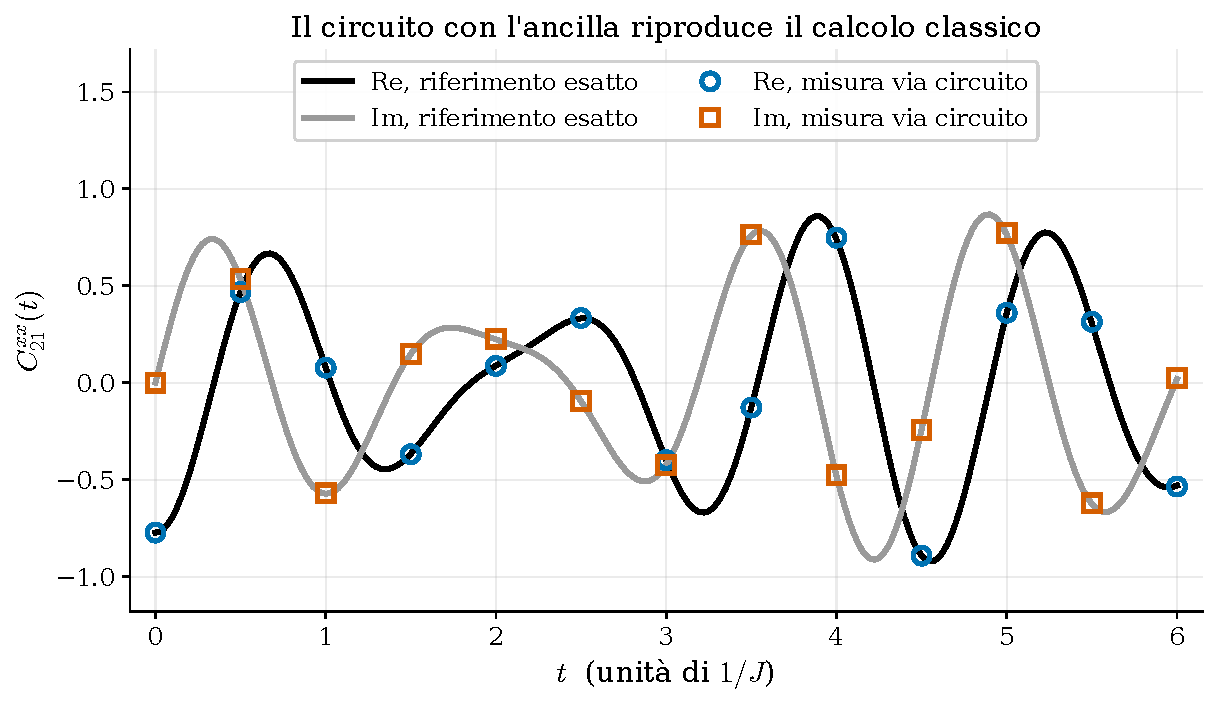
\includegraphics[width=0.86\textwidth]{figure/fig07_correlatore_validazione}
\caption{Un correlatore rappresentativo, su $t\in[0,6]$ (241 punti). Le
curve continue sono il riferimento classico; i simboli sono i valori
estratti dal circuito quantistico. I due si sovrappongono su tutto
l'intervallo, per parte reale e parte immaginaria.}
\end{figure}

\FloatBarrier

\verifica{Il riferimento classico non è calcolato con la stessa formula usata
nel circuito, ma con l'esponenziale di matrice diretta: un'implementazione
indipendente, che non condivide codice con la prima. Il residuo medio è
$4.5\times10^{-3}$, il massimo $1.1\times10^{-2}$, con $N=200$ passi di
Trotter; cresce con $t$, come atteso se l'unica sorgente di discrepanza è la
discretizzazione temporale.}

\needspace{8\baselineskip}
\section{Quali combinazioni vale la pena misurare}

Con due siti e tre componenti le combinazioni sono $36$. Non sono equivalenti:
alcune portano un segnale forte, altre quasi nulla. Vale la pena mapparle tutte
prima di sceglierne una.

\begin{figure}[htbp]
\centering
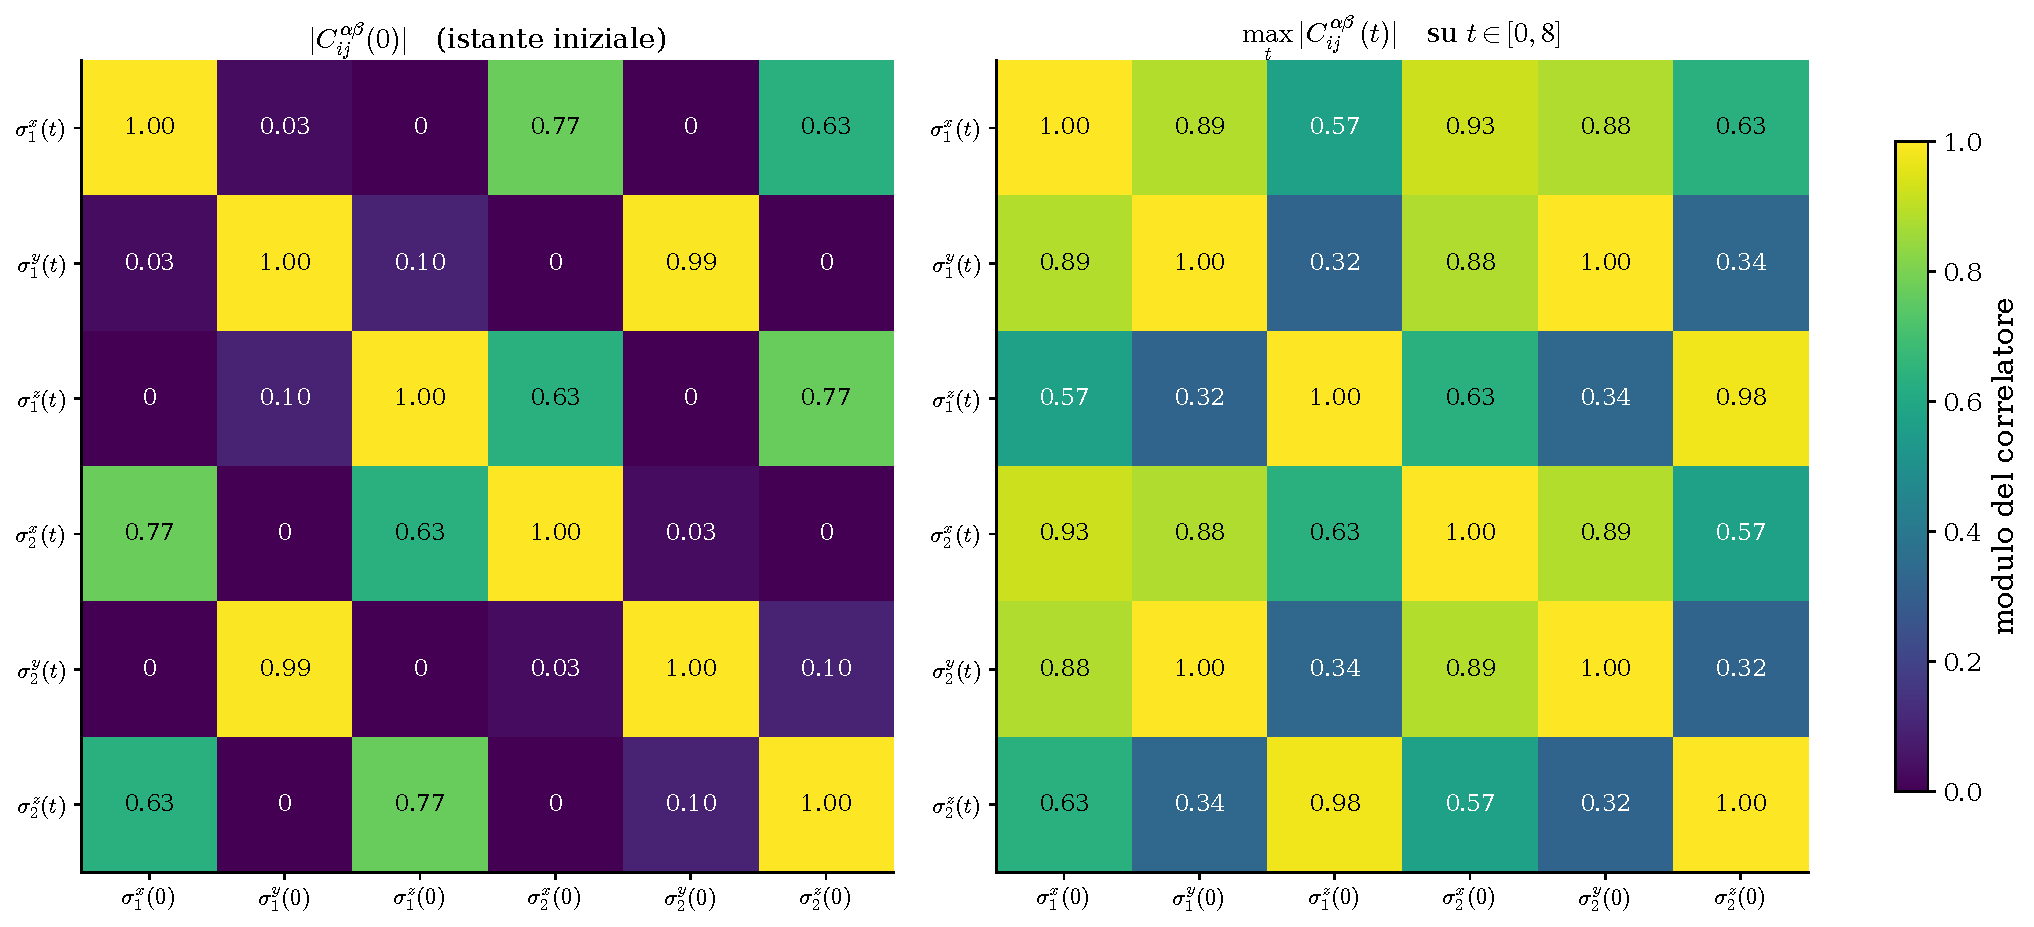
\includegraphics[width=\textwidth]{figure/fig08_scan36}
\caption{Tutte le $36$ combinazioni al punto di lavoro ``test 2''. \textbf{A
sinistra} il valore all'istante iniziale: dodici caselle sono esattamente nulle.
\textbf{A destra} l'ampiezza massima raggiunta su $t\in[0,8]$ (161 punti,
usato per ogni ``$\max_t$'' di questo documento salvo dove dichiarato
altrimenti): nessuna casella
è nulla. Il confronto fra i due pannelli è il risultato: gli zeri sono zeri
\emph{iniziali}, non zeri per ogni tempo. Una combinazione che parte da zero può
comunque diventare un buon segnale, e scartarla guardando solo $t=0$ sarebbe un
errore.}
\label{fig:scan}
\end{figure}

\FloatBarrier

Gli zeri del pannello sinistro hanno una spiegazione a una riga, che si può
enunciare senza calcoli. L'Hamiltoniana del dimero è una matrice reale e
simmetrica, quindi il suo
stato fondamentale si può scegliere reale. Ogni prodotto
$\sigma_i^\alpha\sigma_j^\beta$ che risulti hermitiano ma puramente immaginario
ha allora media nulla su uno stato reale. Sono esattamente due famiglie: le
combinazioni a siti diversi con una sola componente $y$ (otto casi) e le
combinazioni sullo stesso sito con componenti $x$ e $z$ (quattro casi).

\verifica{Le dodici caselle nulle sono verificate numericamente a precisione
macchina, e la classificazione appena data le riproduce tutte e dodici, senza
eccezioni e senza casi in più. Il criterio è quindi predittivo, non una lettura
a posteriori della figura.}

\needspace{10\baselineskip}
\section{Ricco e monocromatico: la stessa fisica vista da angoli diversi}

\begin{figure}[htbp]
\centering

\includegraphics[width=\textwidth]{figure/fig09_ricco_piatto}
\caption{Due correlatori a confronto, sugli stessi assi. A sinistra un
segnale di ampiezza contenuta ma con un battimento visibile, irregolare;
a destra un segnale ampio e perfettamente regolare. Entrambi sono
correlatori legittimi dello stesso sistema nello stesso stato: cambia
solo quali componenti di spin si perturbano e si leggono.}
\end{figure}

\FloatBarrier

La differenza si spiega guardando quali transizioni ciascun correlatore riesce a
eccitare. Vale la pena vederlo esplicitamente, non solo enunciarlo: inserendo
una risoluzione dell'identità nella base degli autostati $\ket{n}$ di $H$
(energie $E_n$, $\ket{0}=\ket{\psi_0}$) fra i due operatori,
\begin{equation}
C_{ij}^{\alpha\beta}(t) = \sum_{n} \underbrace{\bra{0}\sigma_i^\alpha\ket{n}\bra{n}\sigma_j^\beta\ket{0}}_{c_n}\; e^{-i(E_n-E_0)t}.
\end{equation}
Il segnale è dunque \emph{esattamente} una somma di quattro esponenziali
complessi, uno per ciascun autostato $n=0,1,2,3$ (il termine $n=0$ non oscilla:
contribuisce solo alla parte costante). Le grandezze $E_n-E_0$ sono energie,
non frequenze in senso stretto --- ma con $\hbar=1$, la stessa convenzione già
usata per il tempo (in unità di $1/J$), differenza di energia e frequenza
angolare di oscillazione coincidono numericamente: è un'identificazione
esatta, non un abuso di linguaggio. Il peso $c_n$ di ciascuna riga dipende da
quanto bene $\sigma_i^\alpha$ e $\sigma_j^\beta$ collegano il fondamentale a
quel livello --- ed è esattamente ciò che la Fig.~\ref{fig:spettro-righe} più
avanti mostra come istogramma.

\begin{figure}[htbp]
\centering

\includegraphics[width=\textwidth]{figure/fig13_ricostruzione_spettrale}
\caption{Verifica diretta della formula: il segnale calcolato nel modo
consueto (linee continue) confrontato con la somma dei quattro esponenziali
$\sum_n c_n e^{-i(E_n-E_0)t}$ ricostruita dai soli autovalori e autovettori di
$H$ (cerchi). Coincidono a precisione macchina --- lo scarto massimo, indicato
nel titolo di ciascun pannello, è dell'ordine di $10^{-14}$--$10^{-15}$: non è
un'approssimazione che funziona bene, è la stessa identità scritta in due
modi.}
\label{fig:ricostruzione-spettrale}
\end{figure}

\FloatBarrier

\begin{figure}[htbp]
\centering

\includegraphics[width=0.76\textwidth]{figure/fig10_spettro_righe}
\caption{Il peso delle tre transizioni disponibili, per i due correlatori della
figura precedente. Il criterio che distingue i due casi è il rapporto
$a_2/a_1$ fra le due righe più grandi (esclusa $n=0$): $\approx0$ per un
segnale dominato da una sola transizione (monocromatico), $\approx1$ per
transizioni di peso comparabile (segnale ricco). $C_{11}^{yz}$ ha
$a_2/a_1=0.71$ (tre pesi comparabili: $0.170$, $0.049$, $0.121$) --- è
questo, non l'ampiezza, a renderlo ``ricco''. $C_{12}^{zz}$ ha
$a_2/a_1=0.11$: una sola riga concentra il $88\%$ del peso, le altre due
sono quasi trascurabili --- \emph{monocromatico} nel senso spettrale,
anche se la sua ampiezza è la più grande fra tutte le $36$ combinazioni.}
\label{fig:spettro-righe}
\end{figure}

\FloatBarrier

\messaggio{``Ricco'' non significa ampiezza grande --- significa più
transizioni di peso comparabile ($a_2/a_1\approx1$). Un segnale ampio ma
dominato da una sola riga è spettralmente povero, anche se è quello più
facile da misurare. Le due proprietà (ampiezza, ricchezza spettrale) sono
indipendenti, e vanno tenute distinte.}

\needspace{10\baselineskip}
\section{Quando la preparazione non è esatta}

Tutto quanto sopra parte dalle ampiezze esatte di $\ket{\psi_0}$. Ma il
Documento 2 ha già costruito due stati di preparazione veri e propri --- quelli
del VQE --- e alla stessa ``test 2'' le loro fidelity sono molto diverse:
$0.9402$ per l'ansatz base, $1$ (a sei cifre) per quello esteso. Vale la pena
chiedersi cosa succede al correlatore, non solo alla dinamica del Documento 3,
quando la preparazione parte da lì --- usando il correlatore
\emph{spettralmente ricco} appena identificato ($C_{11}^{yz}$,
$a_2/a_1=0.71$), non quello monocromatico: è lì che un errore di
preparazione ha più struttura da perturbare.

\begin{figure}[htbp]
\centering

\includegraphics[width=\textwidth]{figure/fig14_correlatore_da_vqe}
\caption{Il correlatore ``ricco'' $C_{11}^{yz}(t)$, in modulo, su
$t\in[0,8]$: 161 punti per le curve esatte, 41 per il circuito vero
(griglia più rada, per tempo di calcolo con $N=200$ passi di Trotter
ciascuno). Preparato con
due ansatz diversi del Documento 2 e fatto evolvere con il circuito
completo --- ansatz, ancilla, $N=200$ passi di Trotter, transpilato in porte
native. \textbf{A sinistra}, PMA base: la curva esatta da $\psi_{\rm VQE}$
(viola tratteggiata) e il circuito vero (cerchi) sono vicine ma non
identiche --- entrambe seguono lo stesso doppio battimento del riferimento
esatto (nero), con un secondo massimo leggermente sfasato e più alto.
\textbf{A destra}, PMA esteso: la curva esatta e il circuito vero sono
quasi indistinguibili dal riferimento --- per la prima volta si vede
l'errore di Trotter da solo, non più nascosto da un esponenziale esatto
che un circuito reale non potrebbe realizzare.}
\label{fig:correlatore-vqe}
\end{figure}

\FloatBarrier

Lo scarto massimo su $C(t)$ (numero complesso, stessa metrica dello scan
sistematico più avanti), circuito vero incluso, è $0.607$ con l'ansatz
base --- praticamente identico allo scarto della sola preparazione
($0.602$, che coincide esattamente con il valore trovato per questa
combinazione nello scan sistematico), perché anche qui l'errore di
preparazione è molto più grande dell'errore di Trotter. $C_{11}^{yz}$ non
è fra le combinazioni protette: è vicino all'estremo fragile della
distribuzione ($0.053$--$0.64$), coerente con il fatto che coinvolge una
componente $z$. Con l'ansatz esteso lo scarto è $0.019$: non più zero.
Prima, usando l'esponenziale esatto anche per lo stato del VQE, quel
numero sarebbe stato $0$ per costruzione --- un artefatto di aver
chiesto al calcolo qualcosa che un circuito vero non può dare. Con
il circuito vero, l'unico errore rimasto è quello di Trotter --- dentro
l'intervallo trovato nello scan sistematico più avanti
($0.011$--$0.032$).
Lo stesso schema già visto per la dinamica: la conclusione non cambia
spostandosi da una grandezza all'altra, l'errore di preparazione, quando
c'è, domina qualunque cosa si stia misurando a valle --- e ora lo dice un
circuito genuinamente eseguito, non più un calcolo che pretendeva di
esserlo.

Un chiarimento necessario, perché il numero appena dato ($0.602$) sembra
in contrasto con quanto si vede in Fig.~\ref{fig:correlatore-vqe}, dove le
curve in modulo sembrano abbastanza vicine: la Fig.~\ref{fig:correlatore-vqe}
mostra $|C(t)|$, mentre lo scarto $0.602$ è calcolato sul numero
\emph{complesso} $C(t)$ (stessa convenzione dello scan sistematico). Due
numeri complessi possono avere modulo simile ma fase diversa --- ed è
proprio quello che succede qui: l'errore di preparazione sposta
soprattutto la fase del correlatore, un effetto che una figura del solo
modulo non rende visibile per intero.

La forma stessa della curva nera esatta merita uno sguardo, non solo il suo
scarto dal VQE. A differenza di un correlatore monocromatico, qui non c'è
una sola riga dominante: la scomposizione spettrale di
Fig.~\ref{fig:ricostruzione-spettrale} mostra tre pesi comparabili
($c_1=0.170$, $c_2=0.049$, $c_3=0.121$, tutti immaginari puri). Il
battimento più veloce, fra le due righe più pesanti ($E_3-E_1=1.429$,
periodo $2\pi/1.429\approx4.40$), è già visibile sulla curva esatta
stessa: due massimi locali, a $t\approx2.24$ ($|C|=0.32$) e
$t\approx6.62$ ($|C|=0.25$), separati da $4.38$ --- quasi esattamente il
periodo atteso. Non serve un errore di preparazione per vedere un
segnale ricco qui: il fondamentale puro basta da solo, a differenza del
caso monocromatico dove serve un difetto nella preparazione per
introdurre la prima vera struttura di battimento.

L'effetto della preparazione imperfetta, allora, non è \emph{introdurre}
un battimento --- c'è già --- ma \emph{alterarlo}: scomponendo
$\psi_{\rm VQE}$ sugli stessi autostati esatti,
$\psi_{\rm VQE}=0.940\ket0-0.228\ket1+0\cdot\ket2-0.254\ket3$, il peso
mancante rispetto al fondamentale puro ($12\%$) è diviso fra due stati
eccitati diversi, non uno --- e questo introduce nella somma spettrale
un termine di battimento ulteriore fra livelli eccitati
($E_3-E_1=1.429$, la stessa differenza già presente, ma ora con un peso
relativo diverso da quello del fondamentale puro) che sposta l'ampiezza e la
posizione dei massimi rispetto al riferimento esatto --- visibile in
Fig.~\ref{fig:correlatore-vqe} come lo scarto fra la curva nera e quella
viola tratteggiata.

Un solo correlatore, però, non dice se $C_{11}^{yz}$ sia un caso rappresentativo
o un caso sfortunato. Vale la pena rifare lo scan completo di
Fig.~\ref{fig:scan}, questa volta con lo stato del VQE al posto delle
ampiezze esatte, su tutte e $36$ le combinazioni.

\medskip
\noindent\textbf{Esatto.} $e^{-iHt}$ calcolato come esponenziale di matrice
diretto:
\begin{equation*}
C_{\rm esatto}(t) = \bra{\psi}e^{iHt}\,V\,e^{-iHt}\,W\ket{\psi}, \qquad
e^{-iHt} \text{ da \texttt{scipy.linalg.expm}, nessuna approssimazione.}
\end{equation*}
\noindent\textbf{Vero.} Lo stesso correlatore, ma $U(t)$ non è più
l'esponenziale diretto: è il circuito ad ancilla (Fig.~\ref{fig:circ-correlatore})
con $N=200$ passi di Trotter, ciascuno transpilato in porte native
($R_z,\sqrt X,\text{CX}$) ed eseguito porta per porta. Ciò che distingue
``vero'' da ``esatto'' è precisamente questo: nessun circuito reale può
implementare $e^{-iHt}$ in un solo blocco, deve passare da un'approssimazione
a passi discreti.

Qui sotto, i due metodi applicati allo stesso stato prodotto dal VQE ---
imperfetto per l'ansatz base ($\mathcal F=0.940$), praticamente perfetto
per l'esteso ($\mathcal F=1$, a dodici cifre) --- in
due sottosezioni separate, poi confrontati.

\needspace{10\baselineskip}
\subsection*{Primo metodo: il calcolo diretto}

Applicato allo stato prodotto dal VQE invece che a quello esatto:

\begin{figure}[htbp]
\centering
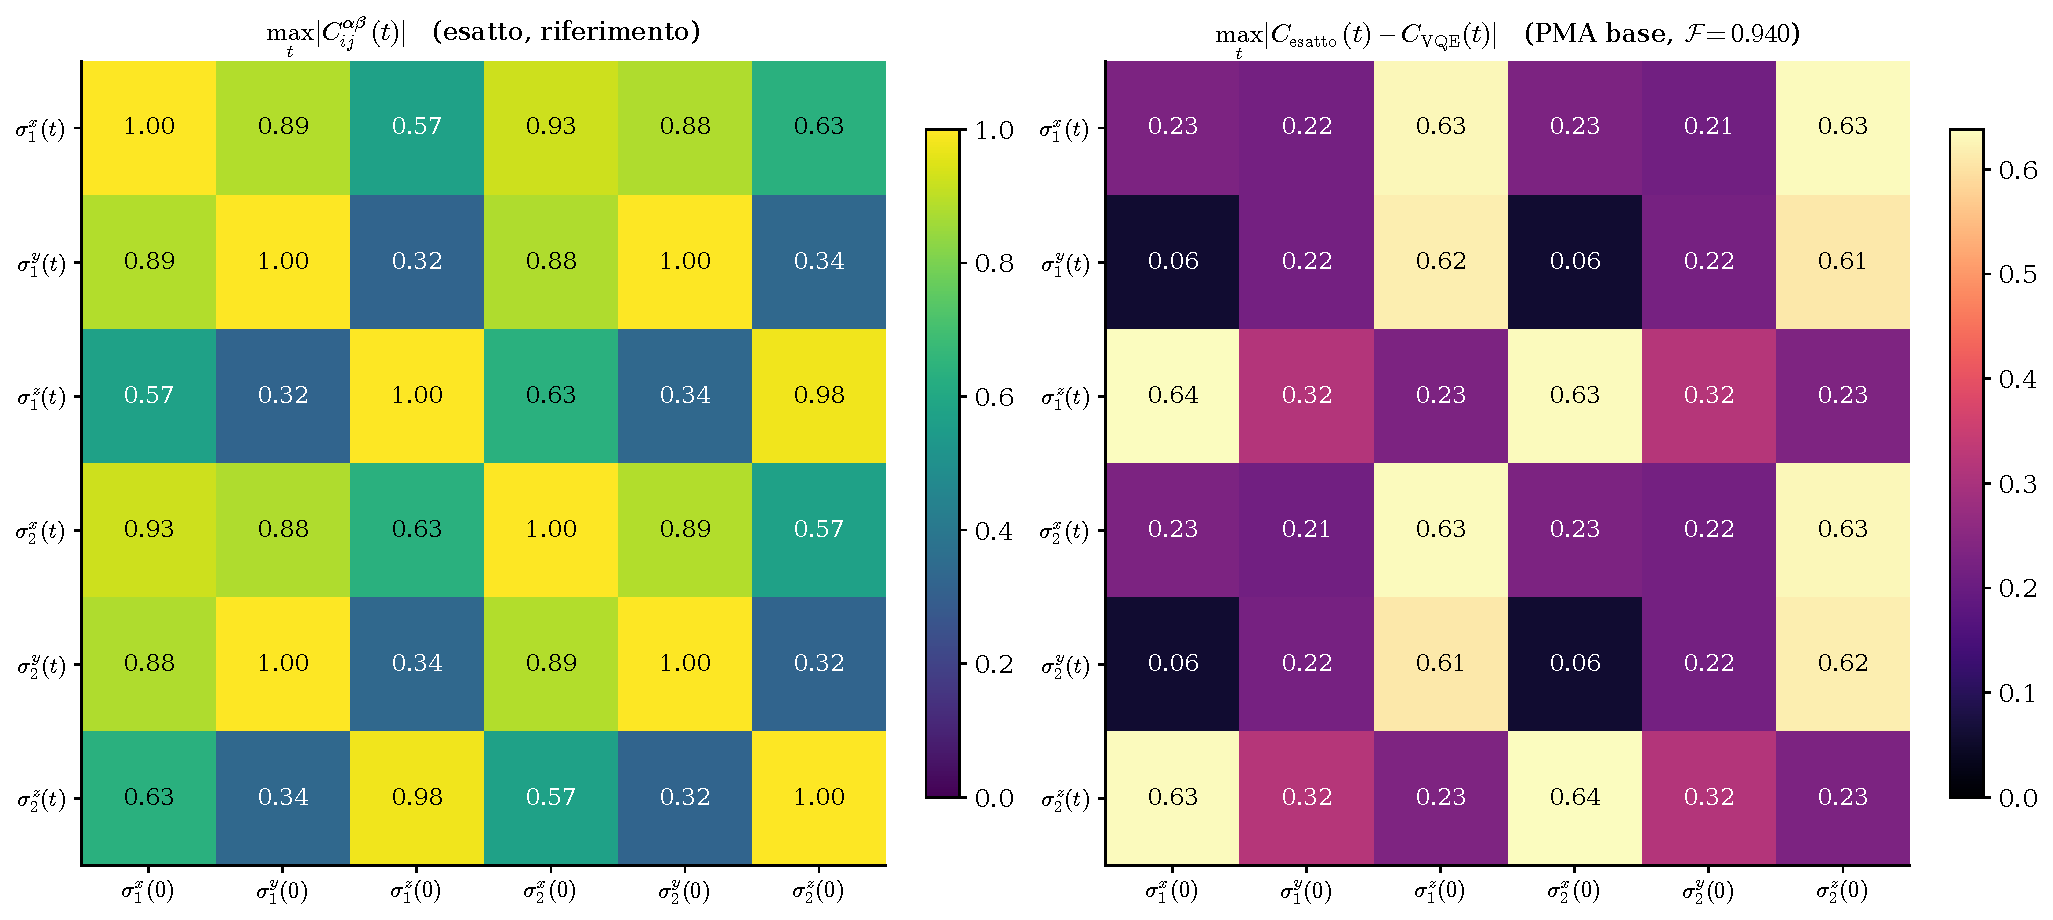
\includegraphics[width=\textwidth]{figure/fig15b_scan36_vqe_diretto}
\caption{\emph{Calcolo diretto} (esponenziale di matrice, non un circuito),
$\max_t$ su $t\in[0,8]$, 161 punti
--- \textbf{a sinistra}, lo stesso riferimento esatto di Fig.~\ref{fig:scan}
(pannello destro). \textbf{A destra}, lo scarto massimo con il PMA base
come preparazione: scarto medio $0.351$, minimo $0.059$, massimo $0.638$
--- fattore $\sim11\times$.}
\label{fig:scan-vqe-diretto}
\end{figure}

\begin{figure}[htbp]
\centering
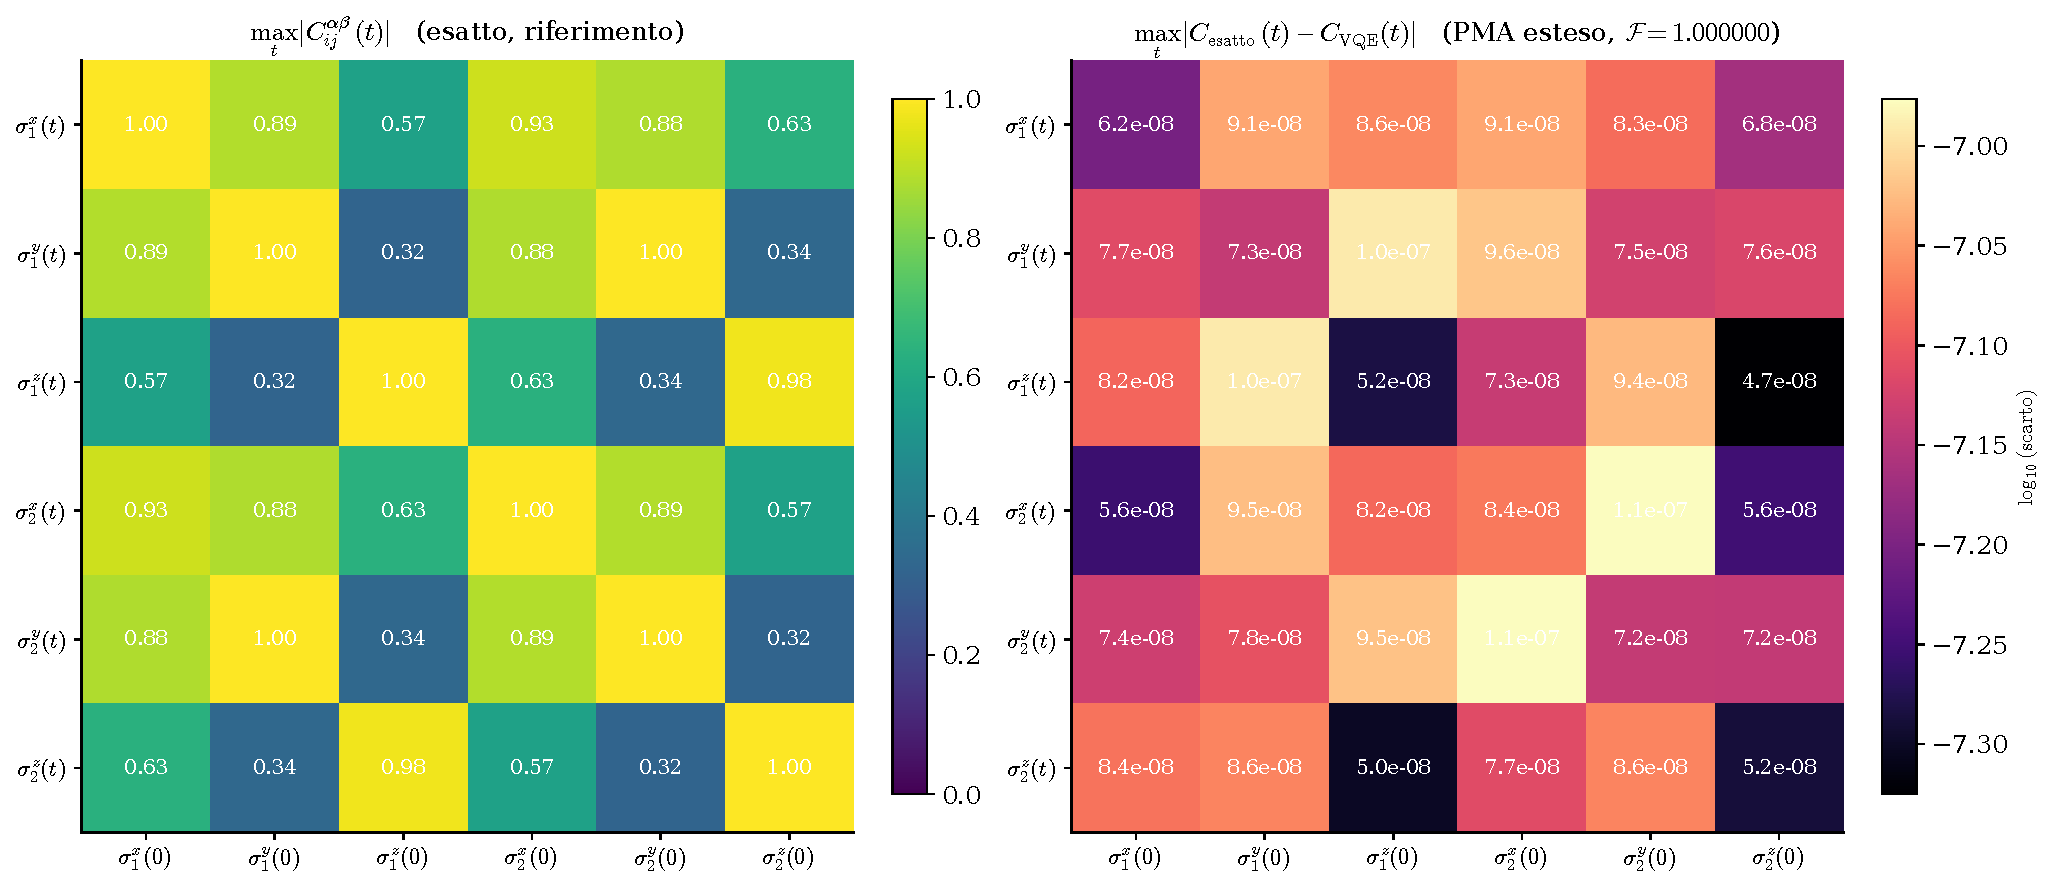
\includegraphics[width=\textwidth]{figure/fig16b_scan36_vqe_esteso_diretto}
\caption{\emph{Calcolo diretto}, stesso metodo e stessa griglia $t\in[0,8]$
(161 punti), con lo stato del PMA
\textbf{esteso}. Scarto uniformemente minuscolo: da $4.7\times10^{-8}$ a
$1.1\times10^{-7}$ --- nessun pattern leggibile, il rapporto fra cella
peggiore e migliore cambia da una corsa di ottimizzazione all'altra.}
\label{fig:scan-vqe-esteso-diretto}
\end{figure}

\FloatBarrier

Con questo metodo, la conclusione per i due ansatz è diversa nella forma:
per il PMA base c'è un pattern strutturale netto e riproducibile; per il
PMA esteso i numeri sono così piccoli da sembrare pura precisione numerica
dell'ottimizzatore, senza nulla di fisico da leggere in una direzione
piuttosto che in un'altra.

\needspace{10\baselineskip}
\subsection*{Secondo metodo: il circuito vero}

Stesso stato del VQE, stessa preparazione:

\begin{figure}[htbp]
\centering

\includegraphics[width=\textwidth]{figure/fig15_scan36_vqe}
\caption{\emph{Circuito vero}, stesso schema della Fig.~\ref{fig:scan-vqe-diretto}
ma con il circuito genuino al posto del calcolo diretto, PMA base ---
$\max_t$ su $t\in[0.1,8]$, \textbf{21 punti} (griglia più rada della
Fig.~\ref{fig:scan-vqe-diretto}, per tempo di calcolo con $N=200$ passi di
Trotter ciascuno; verificato più sotto che non cambia la conclusione). Il
pattern non è uniforme: le combinazioni con una componente $y$ affiancata a
una $x$ (per esempio $\sigma_1^y$--$\sigma_1^x$ o $\sigma_2^y$--$\sigma_2^x$)
restano quasi indenni (scarto $\approx0.05$), mentre le combinazioni miste
$x$--$z$ sono le più fragili (scarto fino a $0.64$) --- coerente con la
struttura del blocco CNOT--$R_y$--CNOT dell'ansatz base (Documento 2,
Fig.~3), che agisce con una rotazione attorno a $y$ e quindi lascia quella
direzione relativamente protetta.}
\label{fig:scan-vqe}
\end{figure}

\begin{figure}[htbp]
\centering
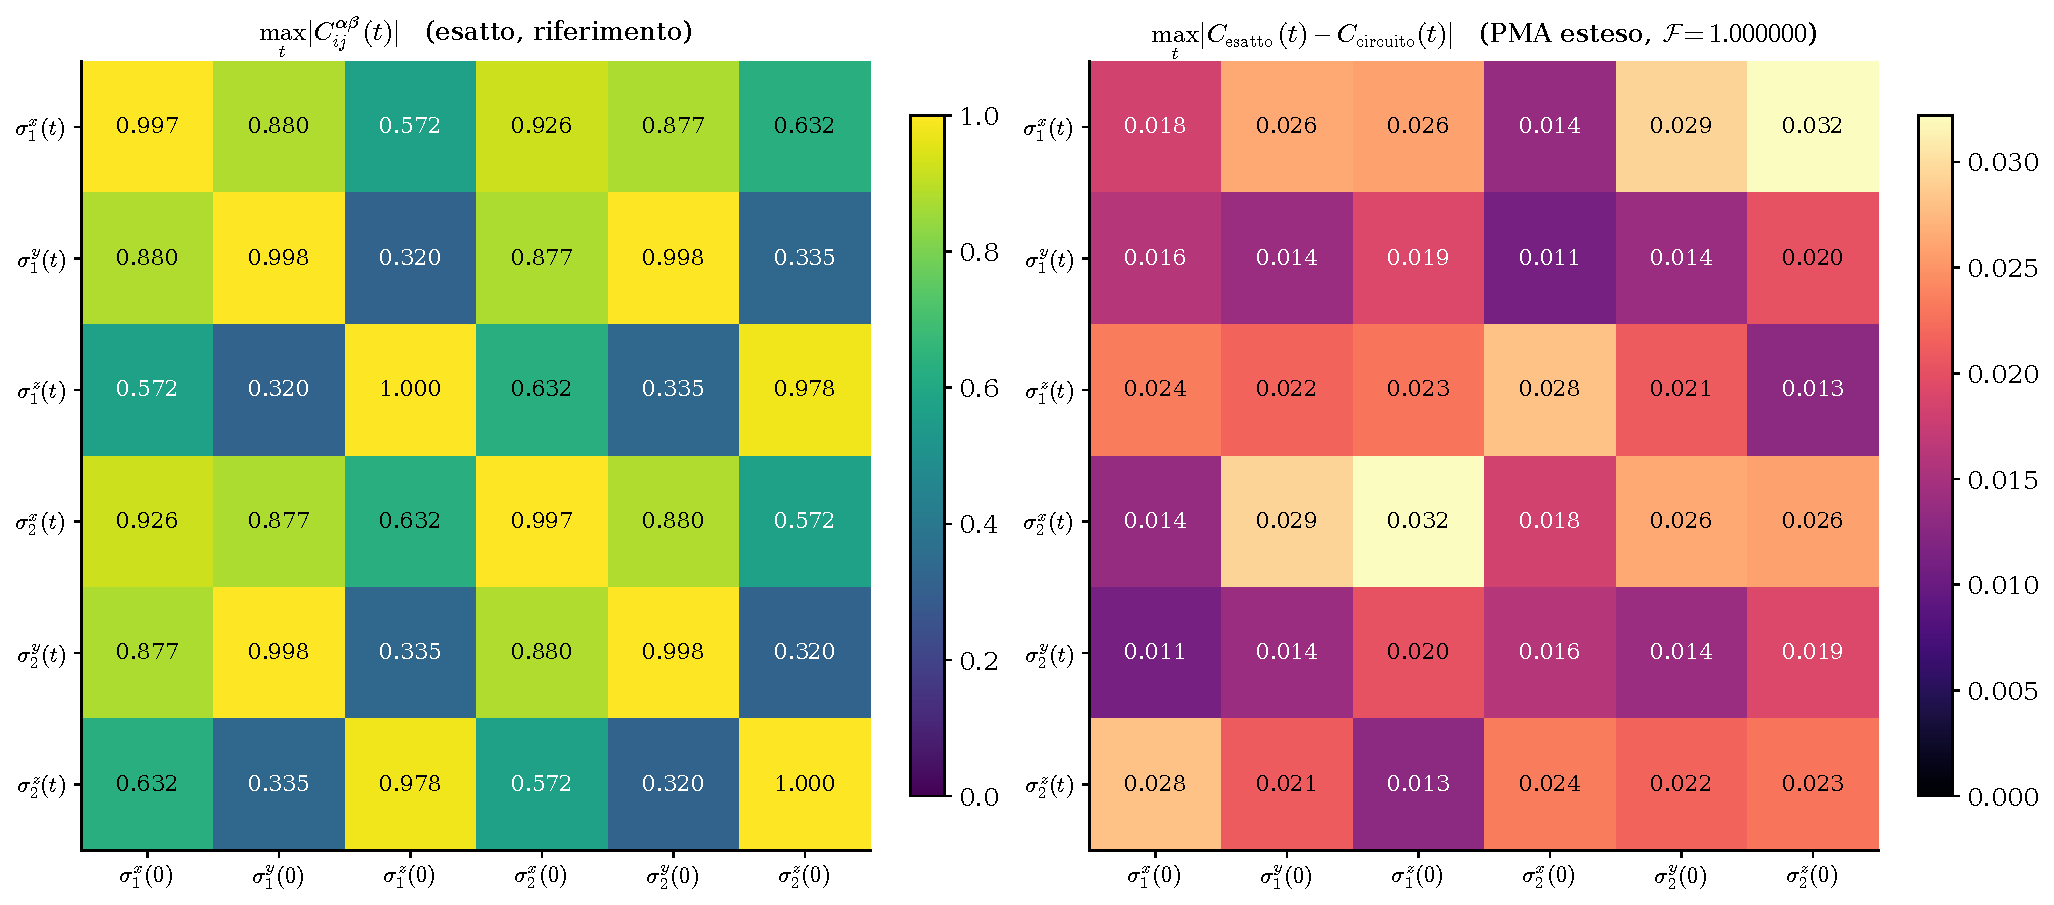
\includegraphics[width=\textwidth]{figure/fig16_scan36_vqe_esteso}
\caption{\emph{Circuito vero}, stesso schema della Fig.~\ref{fig:scan-vqe-esteso-diretto}
ma con il circuito genuino, PMA esteso --- stessa griglia rada $t\in[0.1,8]$,
21 punti. Scala propria (non condivisa con la
Fig.~\ref{fig:scan-vqe}, perché i valori sono un ordine di grandezza più
piccoli): da $0.011$ a $0.032$ --- non più rumore trascurabile, ma un
errore di Trotter reale, con una variazione modesta (circa $3\times$) e
senza il pattern marcato legato alla direzione $y$ visto per il PMA base.}
\label{fig:scan-vqe-esteso}
\end{figure}

\FloatBarrier

Con questo metodo, invece, entrambi gli ansatz mostrano un pattern
leggibile --- marcato per il base, molto più tenue ma presente per
l'esteso: nessuno dei due dà un risultato che assomigli a puro rumore
numerico.

\needspace{10\baselineskip}
\subsection*{Confronto fra i due metodi}

Per il PMA base i due metodi raccontano \textbf{la stessa storia}: scarto
medio $0.351$ (diretto) contro $0.34$ (circuito vero), stesso pattern
strutturale (direzione $y$ protetta), stesso ordine di grandezza ovunque.
Le due griglie temporali sono diverse (161 punti per il calcolo diretto,
21 per il circuito vero, per tempo di calcolo) --- verificato che questo
non cambi la conclusione: sulla combinazione peggiore
($\sigma_1^z$--$\sigma_1^x$), infittendo la griglia del circuito vero da
21 a 81 punti lo scarto passa da $0.641$ a $0.646$, una differenza sotto
l'$1\%$. Il
correlatore $C_{11}^{yz}$ scelto come esempio in
Fig.~\ref{fig:correlatore-vqe} non è fra le combinazioni protette: è
vicino all'estremo fragile della distribuzione, ma non ne è l'estremo
--- vero in entrambi i metodi.

Per il PMA esteso, invece, i due metodi \textbf{non} raccontano la stessa
storia: il calcolo diretto dà uno scarto $10^{-7}$--$10^{-8}$, che assomiglia
a rumore numerico residuo dell'ottimizzatore, senza pattern; il circuito
vero dà $0.011$--$0.032$, quattro-cinque ordini di grandezza più grande, con
una variazione modesta ma reale ($\sim3\times$). La ragione della
differenza: il calcolo diretto confronta due evoluzioni \emph{entrambe}
esatte (l'esponenziale di $H$, applicato sia allo stato vero sia a quello
del VQE) --- un confronto che un circuito reale non può mai realizzare,
perché nessun circuito implementa $e^{-iHt}$ esattamente. Il circuito vero,
passando da Trotter, introduce l'errore che l'esponenziale diretto non può
mostrare per costruzione: non è più zero per lo stato quasi perfetto del
PMA esteso, è il vero errore di evoluzione, coerente con quello già isolato
per $C_{11}^{yz}$ in Fig.~\ref{fig:correlatore-vqe} ($0.019$ su quel
correlatore, dentro l'intervallo $0.011$--$0.032$ trovato qui).

\messaggio{Il metodo di calcolo non è un dettaglio tecnico neutro: per il
PMA base i due metodi concordano, perché l'errore di preparazione domina
qualunque cosa succeda dopo. Per il PMA esteso, dove l'errore di
preparazione è quasi assente, il metodo usato per l'evoluzione temporale
diventa la fonte principale dell'errore residuo --- e un calcolo che
assume un'evoluzione impossibile su hardware reale nasconde esattamente
l'errore che un circuito vero rivelerebbe.}

\section{Che cosa manca, dichiarato}

Tutto quanto sopra è a simulazione ideale. In particolare:

\begin{itemize}[leftmargin=1.5em,itemsep=2pt]
\item L'ancilla è letta sul vettore di stato esatto: non c'è rumore statistico
da numero finito di ripetizioni, né errore di lettura.
\item Non c'è rumore di gate, e il circuito dei correlatori è il più lungo di
tutto il progetto --- contiene $N$ passi di Trotter più le porte controllate.
È quindi il candidato naturale come primo banco di prova quando si introdurrà
il rumore.
\item La preparazione dello stato iniziale, in tutto il documento tranne la
sezione precedente, usa le ampiezze esatte, non il circuito VQE del
Documento 2. La sezione precedente usa lo stato del VQE ovunque, con
\textbf{entrambi} i metodi per l'evoluzione temporale mostrati fianco a
fianco, non uno al posto dell'altro: calcolo diretto ed esponenziale
esatto da un lato, circuito vero (ansatz $+$ ancilla $+$ Trotter)
dall'altro --- per il correlatore singolo
(Fig.~\ref{fig:correlatore-vqe}) e per lo scan sistematico sulle $36$
combinazioni (Fig.~\ref{fig:scan-vqe-diretto}--\ref{fig:scan-vqe-esteso},
per entrambi gli ansatz). Il circuito vero, in particolare, è ormai
verificato ovunque serva confrontarlo con il calcolo diretto: nessun gap
aperto residuo su questo punto. Per le
due topologie a $N=3$ questa chiusura, circuito incluso, è già stata fatta
e validata.
\end{itemize}

\end{document}
